\documentclass[12pt, letterpaper, twoside]{article}    %report   ,  a4paper
\usepackage[utf8]{inputenc}

\title{First document}
\author{Hubert Farnsworth
\thanks{funded by the Overleaf team}}
\date{February 2017}




\usepackage{graphicx}
\graphicspath{ {/} }

% to gre pa potem v tekst    \includegraphics{universe}

%The command \graphicspath{ {images/} } tells LaTeX that the images are kept in a %folder named images under the current directory.

%The \includegraphics{universe} command is the one that actually included the image %in the document. Here universe is the name of the file containing the image %without the extension, then universe.PNG becomes universe. The file name of the %image should not contain white spaces nor multiple dots. 
%Note: The file extension is allowed to be included, but it's a good idea to omit %it. If the file extension is omitted it will prompt LaTeX to search for all the %supported formats. It is also usually recommended to use lowercase letters for the %file extension when uploading image files. 


\begin{document}

\maketitle

We have now added a title, author and date to our first \LaTeX{} document!

Some of the \textbf{greatest}
discoveries in \underline{science} 
were made by \textbf{\textit{accident}}.

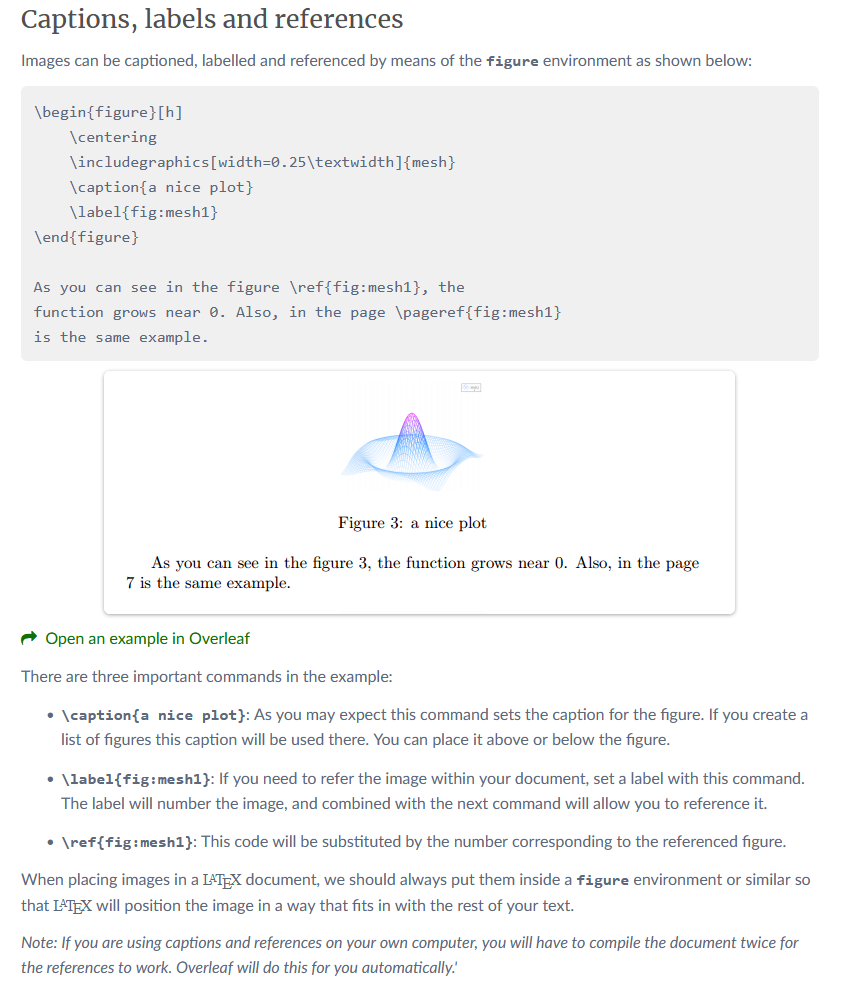
\includegraphics[width=18cm]{ravnanjeSSlikami}

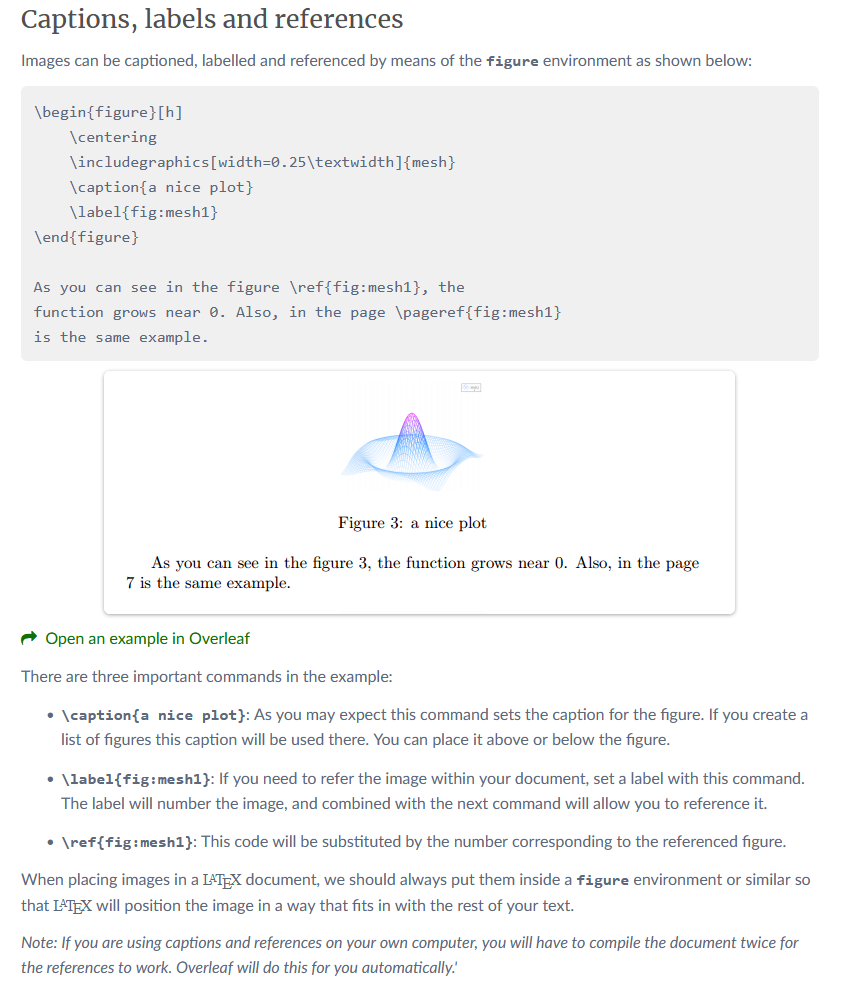
\includegraphics[width=\textwidth]{ravnanjeSSlikami}


\begin{figure}[h]
    \centering
    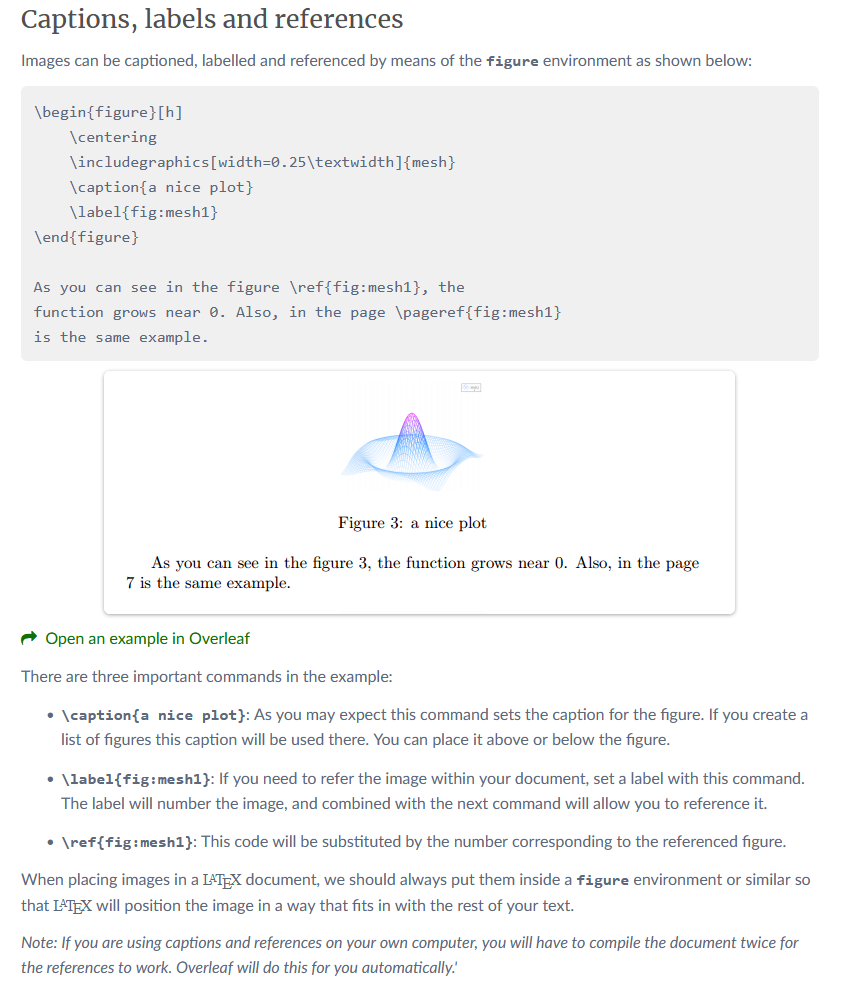
\includegraphics[width=1.25\textwidth]{ravnanjeSSlikami}
    \caption{Instructions}
    \label{fig:inst1}
    
\end{figure}

Good. \ref{fig:inst1}

\end{document}